% Figures of doc/WLZ4_format.md; one page each (build.sh turns page k into the SVG named in figures.txt)
\documentclass[tikz,border=8pt]{standalone}
\usepackage{xcolor}
\pagecolor{white}
\usetikzlibrary{positioning,decorations.pathreplacing,calc,arrows.meta}
% colors and styles shared by the figures of doc/
\definecolor{hdr}{HTML}{FFF2B3}   % size and other headers
\definecolor{tok}{HTML}{C9DCF5}   % tokens, joint symbols
\definecolor{lit}{gray}{0.86}      % literals
\definecolor{off}{HTML}{FAD7B5}   % offset fields
\definecolor{ext}{HTML}{CDEBC7}   % extensions and extra bits
\definecolor{flg}{HTML}{F2A65A}   % flags
\definecolor{endm}{HTML}{F5C2C2}  % end markers
\definecolor{tab}{HTML}{E3D5F2}   % code tables
\definecolor{b1}{HTML}{FBE3CC}    % one, two, three offset bytes
\definecolor{b2}{HTML}{F5BE8A}
\definecolor{b3}{HTML}{E8914A}
\tikzset{
  fld/.style={draw, minimum height=9mm, inner sep=2pt, align=center},
  brc/.style={decorate, decoration={brace, amplitude=4pt}},
  mbrc/.style={decorate, decoration={brace, mirror, amplitude=4pt}}}

\begin{document}

%% 1. wlz4-block: a block and one sequence
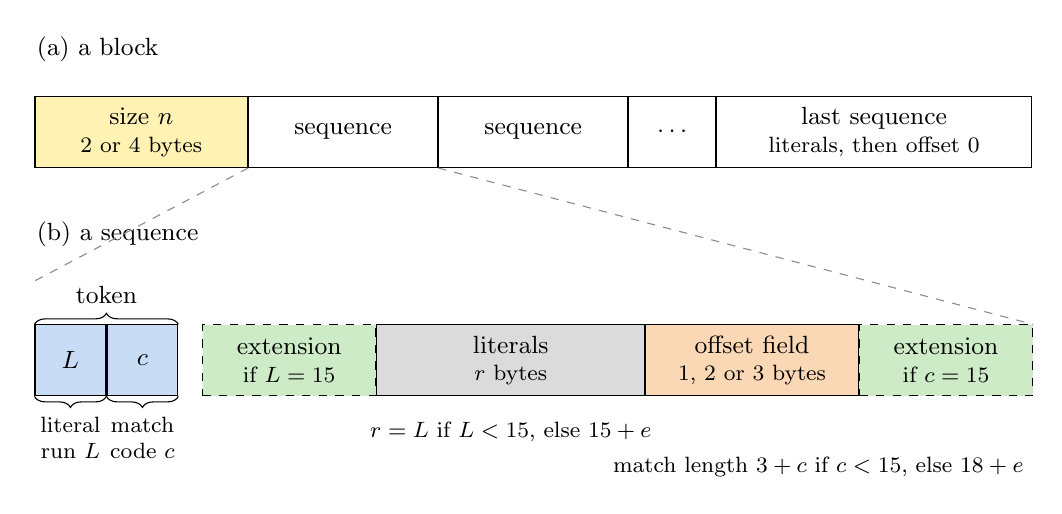
\begin{tikzpicture}[font=\small]
\node[anchor=west] at (-0.1,1.05) {(a) a block};
\node[fld, fill=hdr, minimum width=27mm] (h) at (1.35,0) {size $n$\\[-1pt]\footnotesize 2 or 4 bytes};
\node[fld, minimum width=24mm, right=0pt of h] (s1) {sequence};
\node[fld, minimum width=24mm, right=0pt of s1] (s2) {sequence};
\node[fld, minimum width=11mm, right=0pt of s2] (s3) {$\cdots$};
\node[fld, minimum width=40mm, right=0pt of s3] (s4) {last sequence\\[-1pt]\footnotesize literals, then offset 0};
\node[anchor=west] at (-0.1,-1.3) {(b) a sequence};
\node[fld, fill=tok, minimum width=9mm] (tl) at (0.45,-2.9) {$L$};
\node[fld, fill=tok, minimum width=9mm, right=0pt of tl] (tc) {$c$};
\node[fld, fill=ext, dashed, minimum width=22mm, right=3mm of tc] (le) {extension\\[-1pt]\footnotesize if $L=15$};
\node[fld, fill=lit, minimum width=34mm, right=0pt of le] (li) {literals\\[-1pt]\footnotesize $r$ bytes};
\node[fld, fill=off, minimum width=27mm, right=0pt of li] (of) {offset field\\[-1pt]\footnotesize 1, 2 or 3 bytes};
\node[fld, fill=ext, dashed, minimum width=22mm, right=0pt of of] (me) {extension\\[-1pt]\footnotesize if $c=15$};
\draw[dashed, black!45] (s1.south west) -- ($(tl.north west)+(0,0.55)$);
\draw[dashed, black!45] (s1.south east) -- (me.north east);
\draw[brc] (tl.north west) -- (tc.north east) node[midway, above=4pt] {token};
\draw[mbrc] (tl.south west) -- (tl.south east) node[midway, below=4pt, align=center, font=\footnotesize] {literal\\run $L$};
\draw[mbrc] (tc.south west) -- (tc.south east) node[midway, below=4pt, align=center, font=\footnotesize] {match\\code $c$};
\node[below=2mm of li, font=\footnotesize, align=center] {$r = L$ if $L<15$, else $15+e$};
\node[below=2mm of me.south east, anchor=north east, font=\footnotesize, yshift=-4.5mm] {match length $3+c$ if $c<15$, else $18+e$};
\end{tikzpicture}

%% 2. wlz4-offsets: the offset field of each code, bytes in stream order
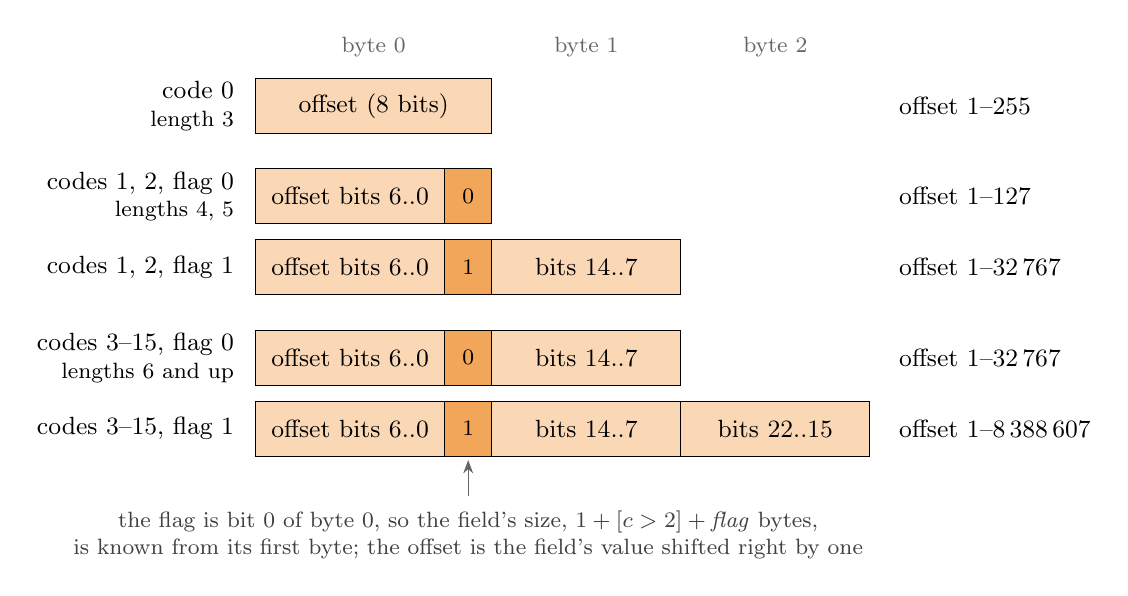
\begin{tikzpicture}[font=\small,
  byte/.style={draw, fill=off, minimum height=7mm, inner sep=1pt, minimum width=24mm},
  flag/.style={draw, fill=flg, minimum height=7mm, inner sep=0pt, minimum width=6mm, font=\footnotesize},
  lab/.style={anchor=east, align=right, font=\small},
  rng/.style={anchor=west, align=left, font=\small}]
\foreach \x/\t in {2.05/byte 0, 4.75/byte 1, 7.15/byte 2} \node[font=\footnotesize, black!60] at (\x,0.75) {\t};
% code 0
\node[lab] at (0.4,0) {code 0\\[-1pt]\footnotesize length 3};
\node[byte, minimum width=30mm] at (2.05,0) {offset (8 bits)};
\node[rng] at (8.6,0) {offset 1--255};
% codes 1-2
\node[lab] at (0.4,-1.15) {codes 1, 2, flag 0\\[-1pt]\footnotesize lengths 4, 5};
\node[byte] at (1.75,-1.15) {offset bits 6..0}; \node[flag] at (3.25,-1.15) {0};
\node[rng] at (8.6,-1.15) {offset 1--127};
\node[lab] at (0.4,-2.05) {codes 1, 2, flag 1};
\node[byte] at (1.75,-2.05) {offset bits 6..0}; \node[flag] at (3.25,-2.05) {1};
\node[byte] at (4.75,-2.05) {bits 14..7};
\node[rng] at (8.6,-2.05) {offset 1--32\,767};
% codes 3-15
\node[lab] at (0.4,-3.2) {codes 3--15, flag 0\\[-1pt]\footnotesize lengths 6 and up};
\node[byte] at (1.75,-3.2) {offset bits 6..0}; \node[flag] at (3.25,-3.2) {0};
\node[byte] at (4.75,-3.2) {bits 14..7};
\node[rng] at (8.6,-3.2) {offset 1--32\,767};
\node[lab] at (0.4,-4.1) {codes 3--15, flag 1};
\node[byte] at (1.75,-4.1) {offset bits 6..0}; \node[flag] at (3.25,-4.1) {1};
\node[byte] at (4.75,-4.1) {bits 14..7};
\node[byte] at (7.15,-4.1) {bits 22..15};
\node[rng] at (8.6,-4.1) {offset 1--8\,388\,607};
\draw[-{Stealth}, black!60] (3.25,-4.95) -- (3.25,-4.5);
\node[font=\footnotesize, align=center, black!75] at (3.25,-5.45) {the flag is bit 0 of byte 0, so the field's size, $1+[c>2]+\mathit{flag}$ bytes,\\is known from its first byte; the offset is the field's value shifted right by one};
\end{tikzpicture}

%% 3. wlz4-windows: the reach of each match length, by offset bytes, against LZ4
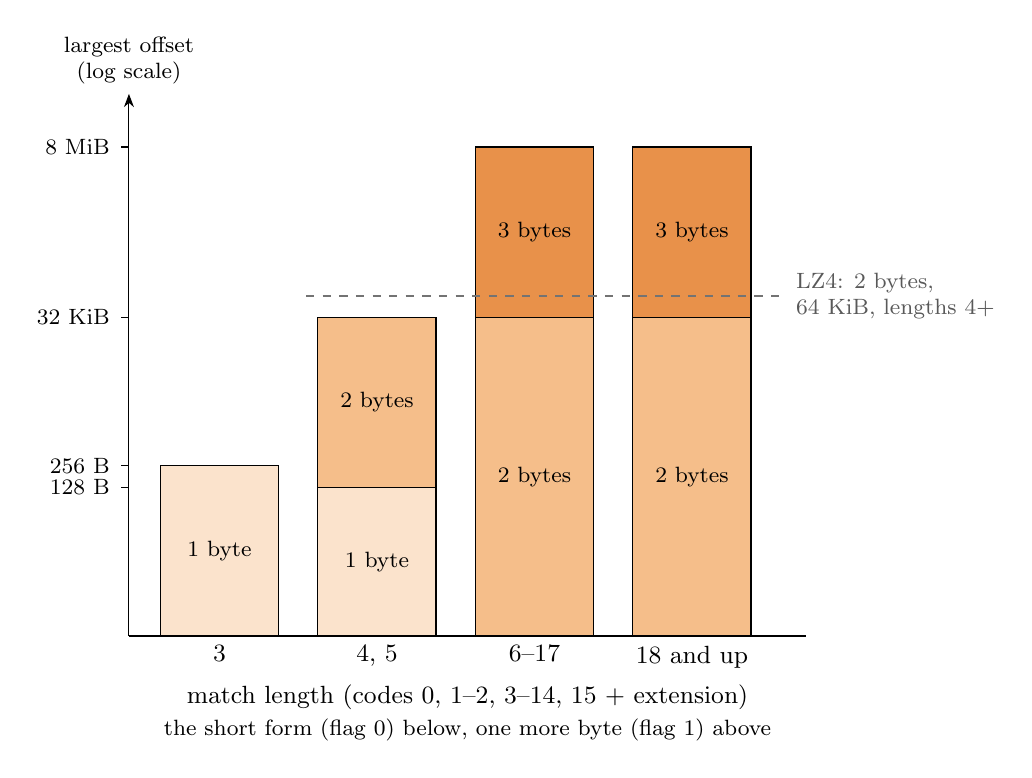
\begin{tikzpicture}[font=\small, y=0.27cm]
\newcommand{\seg}[5]{% x, from (log2), to (log2), fill, label
  \fill[#4] (#1,#2) rectangle ++(1.5,#3-#2);
  \draw (#1,#2) rectangle ++(1.5,#3-#2);
  \node[font=\footnotesize] at (#1+0.75,{(#2+#3)/2}) {#5};}
\draw[-{Stealth}] (0,0) -- (0,25.5) node[above, align=center, font=\footnotesize] {largest offset\\(log scale)};
\draw (0,0) -- (8.6,0);
\foreach \y/\t in {7/128 B, 8/256 B, 15/32 KiB, 23/8 MiB} {
  \draw (-0.1,\y) -- (0,\y);
  \node[anchor=east, font=\footnotesize] at (-0.12,\y) {\t};}
\seg{0.4}{0}{8}{b1}{1 byte}
\seg{2.4}{0}{7}{b1}{1 byte}
\seg{2.4}{7}{15}{b2}{2 bytes}
\seg{4.4}{0}{15}{b2}{2 bytes}
\seg{4.4}{15}{23}{b3}{3 bytes}
\seg{6.4}{0}{15}{b2}{2 bytes}
\seg{6.4}{15}{23}{b3}{3 bytes}
\foreach \x/\t in {1.15/3, 3.15/{4, 5}, 5.15/6--17, 7.15/{18 and up}}
  \node[below, font=\small] at (\x,0) {\t};
\node[below=5mm, font=\small] at (4.3,0) {match length (codes 0, 1--2, 3--14, 15 + extension)};
\draw[dashed, thick, black!55] (2.25,16) -- (8.25,16);
\node[anchor=west, font=\footnotesize, align=left, black!65] at (8.35,16) {LZ4: 2 bytes,\\64 KiB, lengths 4+};
\node[font=\footnotesize, align=center] at (4.3,-4.4) {the short form (flag 0) below, one more byte (flag 1) above};
\end{tikzpicture}

%% 4. wlz4-example: the worked example of section 8
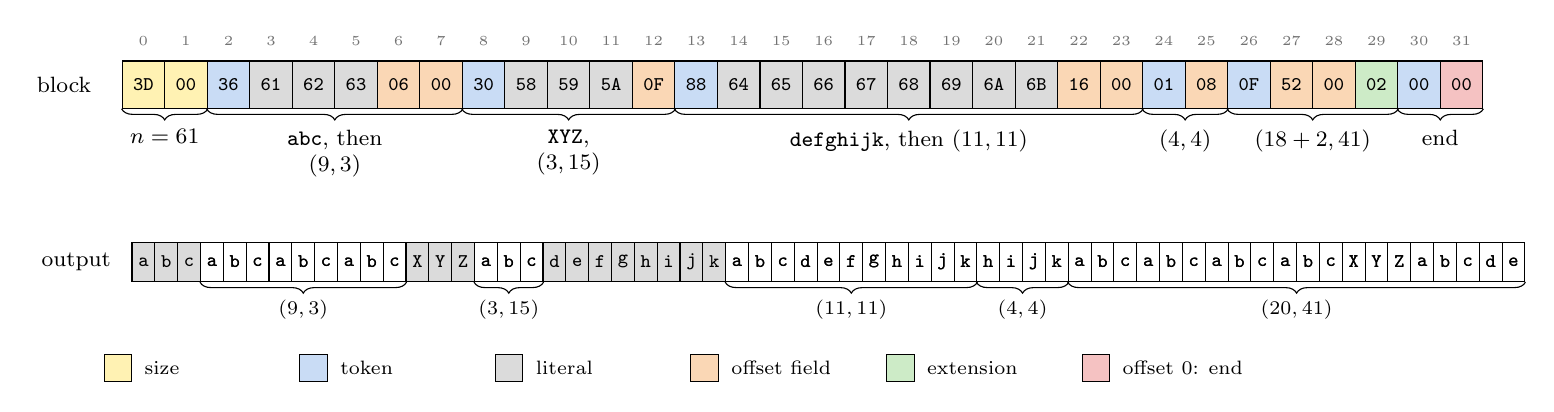
\begin{tikzpicture}[font=\small, x=5.4mm,
  cell/.style={draw, minimum width=5.4mm, minimum height=6mm, inner sep=0pt, font=\ttfamily\scriptsize},
  ocell/.style={draw, minimum width=2.9mm, minimum height=5mm, inner sep=0pt, font=\ttfamily\scriptsize}]
\foreach \b/\k [count=\i from 0] in {3D/hdr,00/hdr, 36/tok,61/lit,62/lit,63/lit,06/off,00/off, 30/tok,58/lit,59/lit,5A/lit,0F/off,
    88/tok,64/lit,65/lit,66/lit,67/lit,68/lit,69/lit,6A/lit,6B/lit,16/off,00/off, 01/tok,08/off, 0F/tok,52/off,00/off,02/ext, 00/tok,00/endm}
  \node[cell, fill=\k] (c\i) at (\i,0) {\b};
\foreach \i in {0,...,31} \node[font=\tiny, black!55] at (\i,0.55) {\i};
\newcommand{\grp}[3]{\draw[mbrc] (c#1.south west) -- (c#2.south east) node[midway, below=4pt, font=\footnotesize, align=center] {#3};}
\grp{0}{1}{$n=61$}
\grp{2}{7}{\texttt{abc}, then\\$(9,3)$}
\grp{8}{12}{\texttt{XYZ},\\$(3,15)$}
\grp{13}{23}{\texttt{defghijk}, then $(11,11)$}
\grp{24}{25}{$(4,4)$}
\grp{26}{29}{$(18+2,41)$}
\grp{30}{31}{end}
% the output
\begin{scope}[x=2.9mm, shift={(0,-2.25)}]
\foreach \ch [count=\i from 0] in {a,b,c,a,b,c,a,b,c,a,b,c,X,Y,Z,a,b,c,d,e,f,g,h,i,j,k,a,b,c,d,e,f,g,h,i,j,k,h,i,j,k,
    a,b,c,a,b,c,a,b,c,a,b,c,X,Y,Z,a,b,c,d,e}
  \node[ocell] (o\i) at (\i,0) {\ch};
\foreach \a/\b in {0/2, 12/14, 18/25} \fill[lit] (o\a.north west) rectangle (o\b.south east);
\foreach \ch [count=\i from 0] in {a,b,c,a,b,c,a,b,c,a,b,c,X,Y,Z,a,b,c,d,e,f,g,h,i,j,k,a,b,c,d,e,f,g,h,i,j,k,h,i,j,k,
    a,b,c,a,b,c,a,b,c,a,b,c,X,Y,Z,a,b,c,d,e}
  \node[ocell] at (\i,0) {\ch};
\newcommand{\cp}[3]{\draw[mbrc] (o#1.south west) -- (o#2.south east) node[midway, below=3pt, font=\scriptsize] {#3};}
\cp{3}{11}{$(9,3)$} \cp{15}{17}{$(3,15)$} \cp{26}{36}{$(11,11)$} \cp{37}{40}{$(4,4)$} \cp{41}{60}{$(20,41)$}
\node[anchor=east, font=\footnotesize] at (-1,0) {output};
\end{scope}
\node[anchor=east, font=\footnotesize] at (-1,0) {block};
\foreach \k/\t [count=\i from 0] in {hdr/size, tok/token, lit/literal, off/offset field, ext/extension, endm/offset 0: end} {
  \node[draw, fill=\k, minimum width=3.5mm, minimum height=3.5mm, inner sep=0pt] at (\i*4.6-0.6,-3.6) {};
  \node[anchor=west, font=\scriptsize] at (\i*4.6-0.2,-3.6) {\t};}
\end{tikzpicture}

\end{document}
